\documentclass[final]{beamer}

\usetheme[subsectionpage=progressbar]{metropolis}
\setbeamertemplate{footline}{}


\usepackage{algorithm2e}
\usepackage{animate}
\usepackage{anyfontsize}
\usepackage[backend=bibtex, style=numeric]{biblatex}
    \addbibresource{references}
\usepackage{booktabs}
\usepackage[font=footnotesize,labelformat=empty]{caption}
\usepackage[default]{Fira Sans}
\usepackage{graphicx}
\usepackage{hyperref}
\usepackage{tikz}
    \usetikzlibrary{%
        arrows.meta,
        decorations.pathreplacing,
        decorations.text,
        patterns,
        shapes.arrows,
        shapes.geometric
    }


% TikZ styles, commands and settings
\definecolor{cyan}{RGB}{0, 164, 216}
\definecolor{magenta}{RGB}{226, 62, 138}
\tikzstyle{every picture} += [remember picture]
\tikzstyle{na} = [baseline=-.5ex]

\tikzset{%
    column/.pic={%
        code{%
            \draw[line width=1pt] (0, 0) rectangle (-2cm, 4cm);
            \foreach \val in {0, ..., #1}{%
                \draw[rotate=90] ([xshift=-\val*10pt] 4cm, 2cm) -- ++(0, -2cm);
            };
            \node at (-1cm, 1.25) {$\vdots$};
            \foreach \val in {1, 2}{%
                \draw (0, \val * 10pt) -- ++(-2cm, 0);
            };
        }
    }
}

\tikzset{%
    fullcolumn/.pic={%
        code{%
            \draw[line width=1pt] (0, 0) rectangle (-2cm, #1*10pt);
            \foreach \val in {0, ..., #1}{%
                \draw[rotate=90] ([xshift=-\val*10pt] #1*10pt, 2cm) -- ++(0, -2cm);
            };
        }
    }
}

\newcommand{\hammerpage}{%
    \frame{%
        \centering
        \includegraphics[width=.2\textwidth]{img/nut.png}\hspace{.1\textwidth}%
        \includegraphics[width=.5\textwidth]{img/hammer.png}
    }
}

\title{%
    Evolutionary dataset optimisation:
    learning algorithm quality through evolution
}
\author{\large{Henry Wilde, Dr.\ Jonathan Gillard, Dr.\ Vincent Knight}}
\institute{%
    \vfill%
    \centering%
    \includegraphics[height=.2\paperheight]{img/cu_logo.png}%
    \hspace{5pt}%
    \includegraphics[height=.2\paperheight]{img/cthb_logo.jpg}
}
\date{}

\begin{document}

\frame{%
    \maketitle%
}

\frame{%
    \centering
    \begin{figure}
        \includegraphics[width=.8\textwidth]{../img/gorilla.png}
        \caption{%
            via: BBC News (\url{%
                https://www.bbc.co.uk/news/technology-33347866
            })
        }
    \end{figure}
}

\frame{%
    \centering
    \resizebox{!}{.9\paperheight}{%
        \begin{tikzpicture}

    \begin{pgfonlayer}{background}
    % Data
    \node[%
        ellipse,
        minimum height=3cm,
        minimum width=7cm,
        fill=cyan!15,
        label={below:\Large Data}
        ] at (0, 0) {};

    % Algorithms
    \node[%
        rectangle,
        rounded corners=0.25cm,
        minimum height=1cm,
        minimum width=6cm,
        fill=orange!15,
        label={\Large Algorithms}
    ] at (0, -6) {};
    \end{pgfonlayer}

    \pause
    \node[circle, fill=cyan, thick, inner sep=2pt, minimum size=2mm]
        (d) at (2, 0) {};

    \pause
    \node[circle] (q1) at (2, -2) {?};
    \draw[->, thick] (d.south) -- (q1.north);

    \pause
    \node[circle] (q2a) at (1, -3) {?};
    \node[circle] (q2b) at (3, -3) {?};
    \draw[->, thick] (q1.south west) -- (q2a.north east);
    \draw[->, thick] (q1.south east) -- (q2b.north west);

    \pause
    \node[circle] (q3) at (2, -4) {?};
    \draw[->, thick] (q2a.south east) -- (q3.north west);
    \draw[thick] (q2a.south west) -- ++(-0.5, -0.5);

    \pause
    \node[circle, fill=orange, thick, inner sep=2pt, minimum size=2mm]
        (a) at (2, -6) {};

    \draw[->, thick] (q3.south) -- (a.north);

    \pause
    \node[circle, fill=orange, thick, inner sep=2pt, minimum size=2mm]
        (a2) at (-2, -6) {};

    \pause
    \node[%
        ellipse,
        fill=cyan!50,
        minimum height=0.75cm,
        minimum width=1cm
    ] (datasets) at (-1.5, 0) {};
    \foreach \position in {(-1.7, 0), (-1.5, 0.1), (-1.3, -0.1)} {%
        \fill[cyan] \position circle (1mm);
    };

    \pause
    \node[%
        ellipse,
        fill=cyan!35,
        minimum height=1.3cm,
        minimum width=2.5cm,
    ] (data) at (-1, 0) {};

    \node[%
        ellipse,
        fill=cyan!50,
        minimum height=0.75cm,
        minimum width=1cm
    ] (datasets) at (-1.5, 0) {};
    \foreach \position in {(-1.7, 0), (-1.5, 0.1), (-1.3, -0.1)} {%
        \fill[cyan] \position circle (1mm);
    };

    \pause
    \draw[->, thick]
        (a2.north west) to [out=130, in=210] (data.south west);
\end{tikzpicture}

    }
}

\section{Generating artificial data}

\frame{%
    \centering
    \begin{figure}
        \includegraphics[width=.3\textwidth]{../img/faces/0.jpeg}\hfill%
        \includegraphics[width=.3\textwidth]{../img/faces/1.jpeg}\hfill%
        \includegraphics[width=.3\textwidth]{../img/faces/2.jpeg}
        \caption{via: \url{https://thispersondoesnotexist.com}}
    \end{figure}
}

\frame{%
    \alert{Anscombe's quartet}\vfill
    \includegraphics[width=\textwidth]{../img/anscombes.pdf}\vfill
}

\frame{%
    \resizebox{\textwidth}{!}{%
        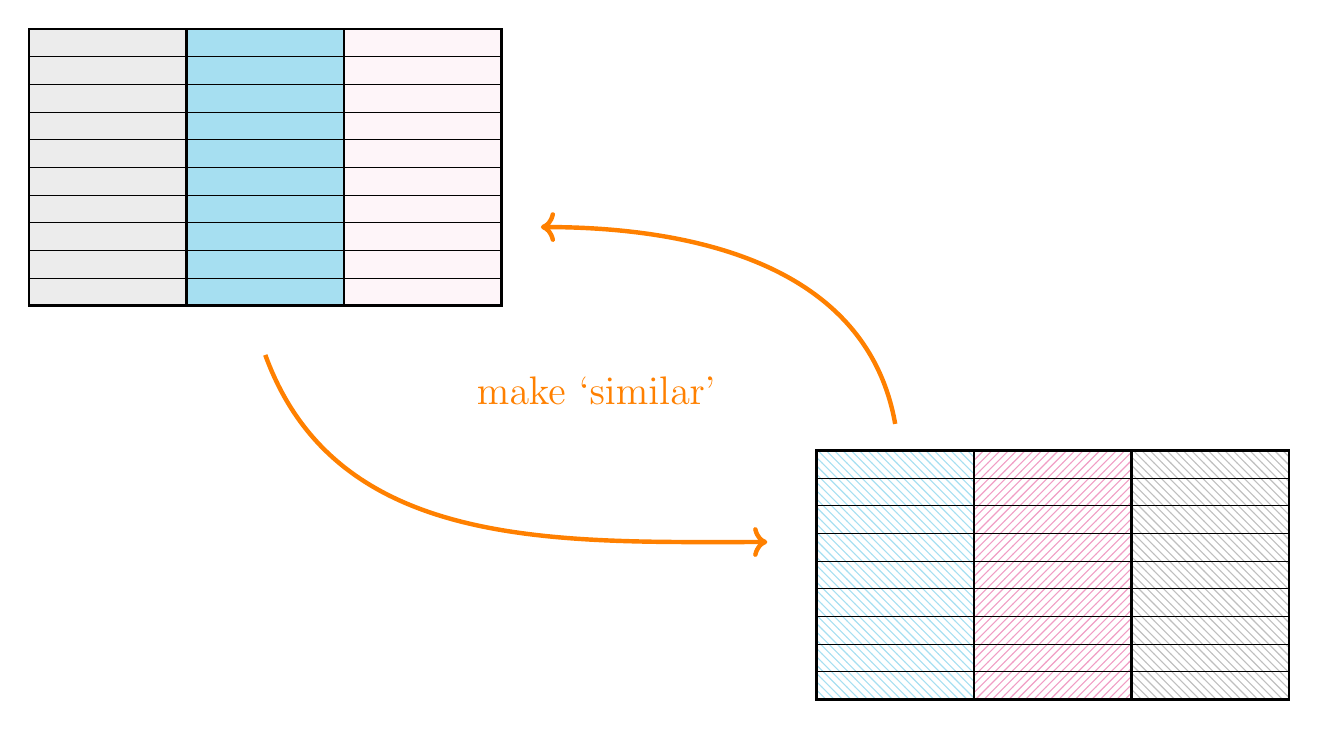
\begin{tikzpicture}

    % Dataset
    \fill[gray!15] (-4, 5) rectangle (-2, 8.5);
    \fill[cyan!35] (-2, 5) rectangle (0, 8.5);
    \fill[magenta!5] (0, 5) rectangle (2, 8.5);
    \path (-2, 5) pic {fullcolumn=10}
          (0, 5) pic {fullcolumn=10}
          (2, 5) pic {fullcolumn=10};
    \node (dataset) at (-1, 4.5) {};

    % A similar dataset
    \fill[pattern=north west lines, pattern color=cyan!35]
        (6, 0) rectangle (8, 3.15);
    \fill[pattern=north east lines, pattern color=magenta!50]
        (8, 0) rectangle (10, 3.15);
    \fill[pattern=north west lines, pattern color=gray!50]
        (10, 0) rectangle (12, 3.15);
    \path (8, 0) pic {fullcolumn=9}
        (10, 0) pic {fullcolumn=9}
        (12, 0) pic {fullcolumn=9};
    \node (similar) at (5.5, 2) {};

    \draw[->, orange, ultra thick]
        (dataset.south) to [out=290, in=180] (similar.west);
    \draw[->, orange, ultra thick]
        (7, 3.5) to [out=100, in=0] (2.5, 6) node[right=20pt, below=50pt]
        {\Large\color{orange} make `similar'};

\end{tikzpicture}

    }
}

\frame{%
    \huge{%
        Given an algorithm, how can one find sets of data for which it performs
        well?
    }
}


\section{Evolutionary algorithms}

\frame{%
    \resizebox{\textwidth}{!}{%
        \input{tex/flowchart.tex}
    }
}

\frame{%
    \[
        \max\quad f: \mathbb{N}^2 \to \mathbb{N}; \qquad f(x_1, x_2) = x_1 + x_2
    \]\vfill
    \begin{tabular}{lccccc}
        \pause%
        \alert{Population} & (25, 30) & (12, 1) & (11, 0) & (20, 12) & (24, 25)\\\\
        \pause%
        \alert{Get fitness} & 55 & 13 & 11 & 42 & 49\\\\
        \pause%
        \alert{Select parents} & (25, 30) & {} & {} & (20, 12) & (24, 25)\\\\
        \pause%
        \alert{Create offspring} & & (24, 30) & (25, 12) & & \\\\
        \pause%
        \alert{Mutate offspring} & & (\alert{15}, 30) & (25, \alert{26}) & & \\\\
        \pause%
        \alert{New generation} & (25, 30) & (15, 30) & (25, 26) & (20, 12) & (24, 25)
    \end{tabular}
}

\frame{%
    \tiny{%
    \begin{itemize}
        \item A fitness function, \(f\), which acts on a single dataset
        \item A population size, \(N \in \mathbb{N}\)
        \item A maximum number of iterations, \(M \in \mathbb{N}\)
        \item A selection parameter to detail the proportion of the
            fittest individuals to carry forward, \(b \in [0, 1]\)
        \item A mutation probability, \(p_m \in [0, 1]\)
    \end{itemize}
    \vspace{-10pt}\noindent\rule{\linewidth}{0.4pt}\vspace{-10pt}
    \begin{itemize}
        \item Limits on the number of rows a dataset can have:
            \[
                R \in \left\{%
                    (r_{\min}, r_{\max})
                    \in \mathbb{N}^2~|~r_{\min} \leq r_{\max}
                \right\}
            \]
        \item Limits on the number of columns a dataset can have:
            \[
                C := \left(C_1, \ldots, C_{|\mathcal{P}|}\right)
                ~\text{where}~
                C_j \in \left\{ (c_{\min}, c_{\max}) \in {%
                    \left(\mathbb{N}\cup\{\infty\}\right)
                }^2~|~c_{\min} \leq c_{\max}\right\}
            \]
            for each \(j = 1, \ldots, |\mathcal{P}|\)
        \item A set of probability distribution families, \(\mathcal{P}\). Each
            family in this set has some parameter limits which form a part of
            the overall search space
        \item A probability vector to sample distributions from \(\mathcal{P}\),
            \(w = \left(w_1, \ldots, w_{|\mathcal{P}|}\right)\)
        \item A second selection parameter, \(l \in [0, 1]\), to allow for a
            small proportion of ``lucky'' individuals to be carried forward
        \item A shrink factor, \(s \in [0, 1]\). The relative size of a
            component of the search space to be retained after adjustment
    \end{itemize}
    }
}

\frame{%
    \vfill\alert{Individuals}\vfill
    \resizebox{\textwidth}{!}{%
        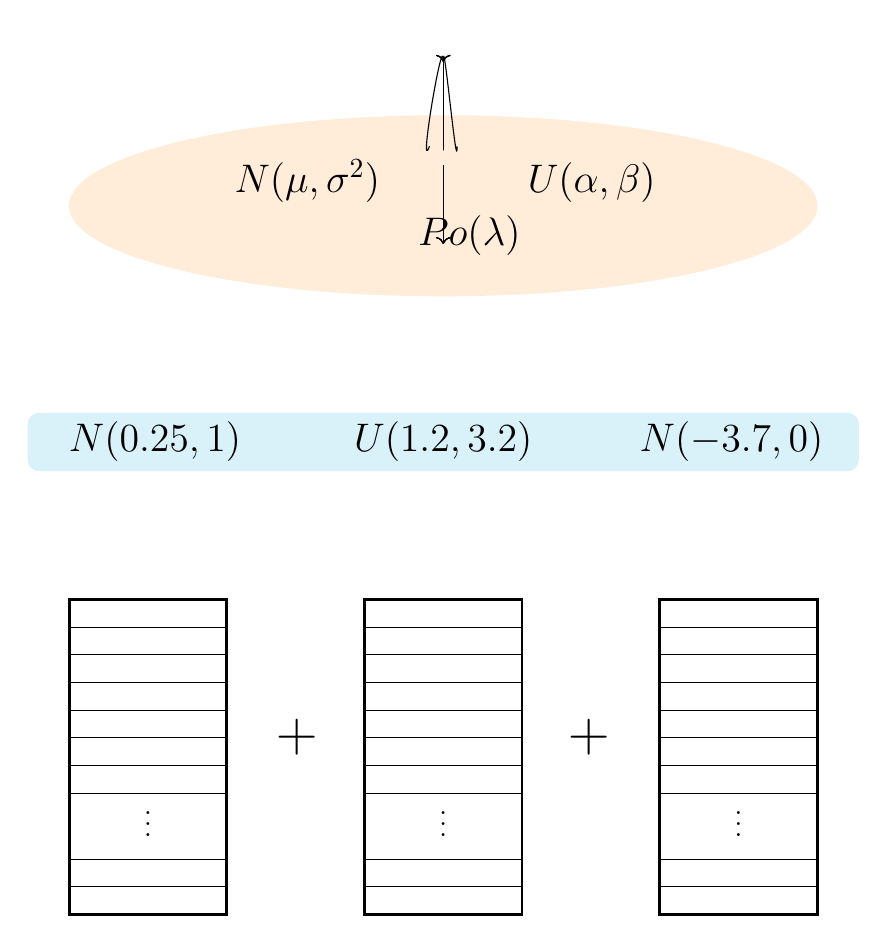
\begin{tikzpicture}

    % Columns
    \path (-2.75, -10) pic {column=7}
          (1, -10) pic {column=7}
          (4.75, -10) pic {column=7};

    \node at (-1.85, -7.75) {\huge \(+\)};
    \node at (1.85, -7.75) {\huge \(+\)};

    % Distribution families
    \node[ellipse, fill=orange!15] (dists) at (0, -1) {\Large%
        \begin{tabular}{c}
            \tikz[baseline, inner sep=0] \node[anchor=base] (normal)
                {\(N(\mu, \sigma^2)\)};
            \qquad
            \tikz[baseline, inner sep=0] \node[anchor=base] (uniform)
                {\(U(\alpha, \beta)\)};
            \\
            {} \quad \(Po(\lambda)\)
        \end{tabular}
    };

    % Metadata
    \node[fill=cyan!15, minimum width=3cm, rounded corners] (metadata) at
        (0, -4) {\Large%
            \tikz[baseline, inner sep=0] \node[anchor=base] (norm1)
                {\(N(0.25, 1)\)};
            \quad
            \tikz[baseline, inner sep=0] \node[anchor=base] (uniform1)
                {\(U(1.2, 3.2)\)};
            \quad
            \tikz[baseline, inner sep=0] \node[anchor=base] (norm2)
                {\(N(-3.7, 0)\)};
        };
 
    % Connecting family to metadata
    \draw[->] ([xshift=-5pt] normal.south)
        to [out=250, in=90] ([yshift=20pt] norm1);

    \draw[->] (uniform) to [out=270, in=90] ([yshift=20pt] uniform1);

    \draw[->] ([xshift=5pt] normal.south)
        to [out=270, in=90] ([yshift=20pt] norm2);

    % Connecting metadata to columns
    \draw[->] ([yshift=-10pt] norm1.south) -- ++(0, -1);
    \draw[->] ([yshift=-10pt] uniform1.south) -- ++(0, -1);
    \draw[->] ([yshift=-10pt] norm2.south) -- ++(0, -1);

\end{tikzpicture}

    }\vfill
}

\frame{%
    \vfill\alert{Selection}\vfill
    \centering
    \resizebox{!}{.75\paperheight}{%
        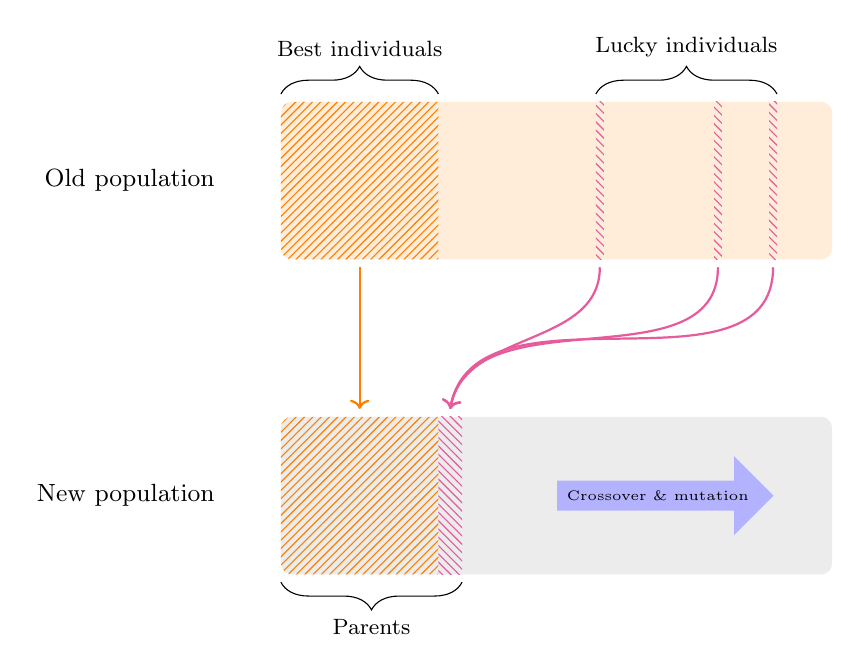
\begin{tikzpicture}

    \fill[orange!15, rounded corners] (0, 0) rectangle (7, 2)
    node[left=120pt, midway] {\small{\color{black} Old population}};
    \fill[rounded corners, gray!15] (0, -4) rectangle (7, -2)
    node[left=120pt, midway] {\small{\color{black} New population}};

    \fill[pattern=north east lines, pattern color=orange]
        (2, 0) --
        ++(0, 2) {[rounded corners] --
        ++(-2, 0) --
        ++(0, -2)} --
        cycle
        {};
   
    \draw[->, orange, thick] (1, -0.1) to (1, -1.9);

    \fill[pattern=north east lines, pattern color=orange]
        (2, -4) --
        ++(0, 2) {[rounded corners] --
        ++(-2, 0) --
        ++(0, -2)} --
        cycle
        {};

    \foreach \val in {4, 5.5, 6.2} {%
        \fill[pattern=north west lines, pattern color=magenta!85]
            (\val, 0) rectangle (\val+0.1, 2);
        \draw[->, magenta!85, thick]
            (\val+0.05, -0.1) to [out=270, in=80] (2.15, -1.9);
    };

    \fill[pattern=north west lines, pattern color=magenta!85]
        (2, -4) rectangle (2.3, -2);

    \draw[decorate, decoration={brace, amplitude=10pt}] (0, 2.1) -- (2, 2.1)
        node[midway, above=10pt] {\footnotesize{Best individuals}};
    \draw[decorate, decoration={brace, amplitude=10pt}] (4, 2.1) -- (6.3, 2.1)
        node[midway, above=10pt] {\footnotesize{Lucky individuals}};
    \draw[decorate, decoration={brace, amplitude=10pt}] (2.3, -4.1) -- (0, -4.1)
        node[midway, below=10pt] {\footnotesize{Parents}};

    \node[%
        fill=blue!30, single arrow, minimum height=20mm, minimum width=10mm,
        single arrow head extend=3mm, anchor=west
    ] at (3.5, -3) {\tiny{Crossover \& mutation}};

\end{tikzpicture}

    }\vfill
}

\frame{%
    \vfill\alert{Crossover}\vfill
    \centering
    \resizebox{!}{.65\paperheight}{%
        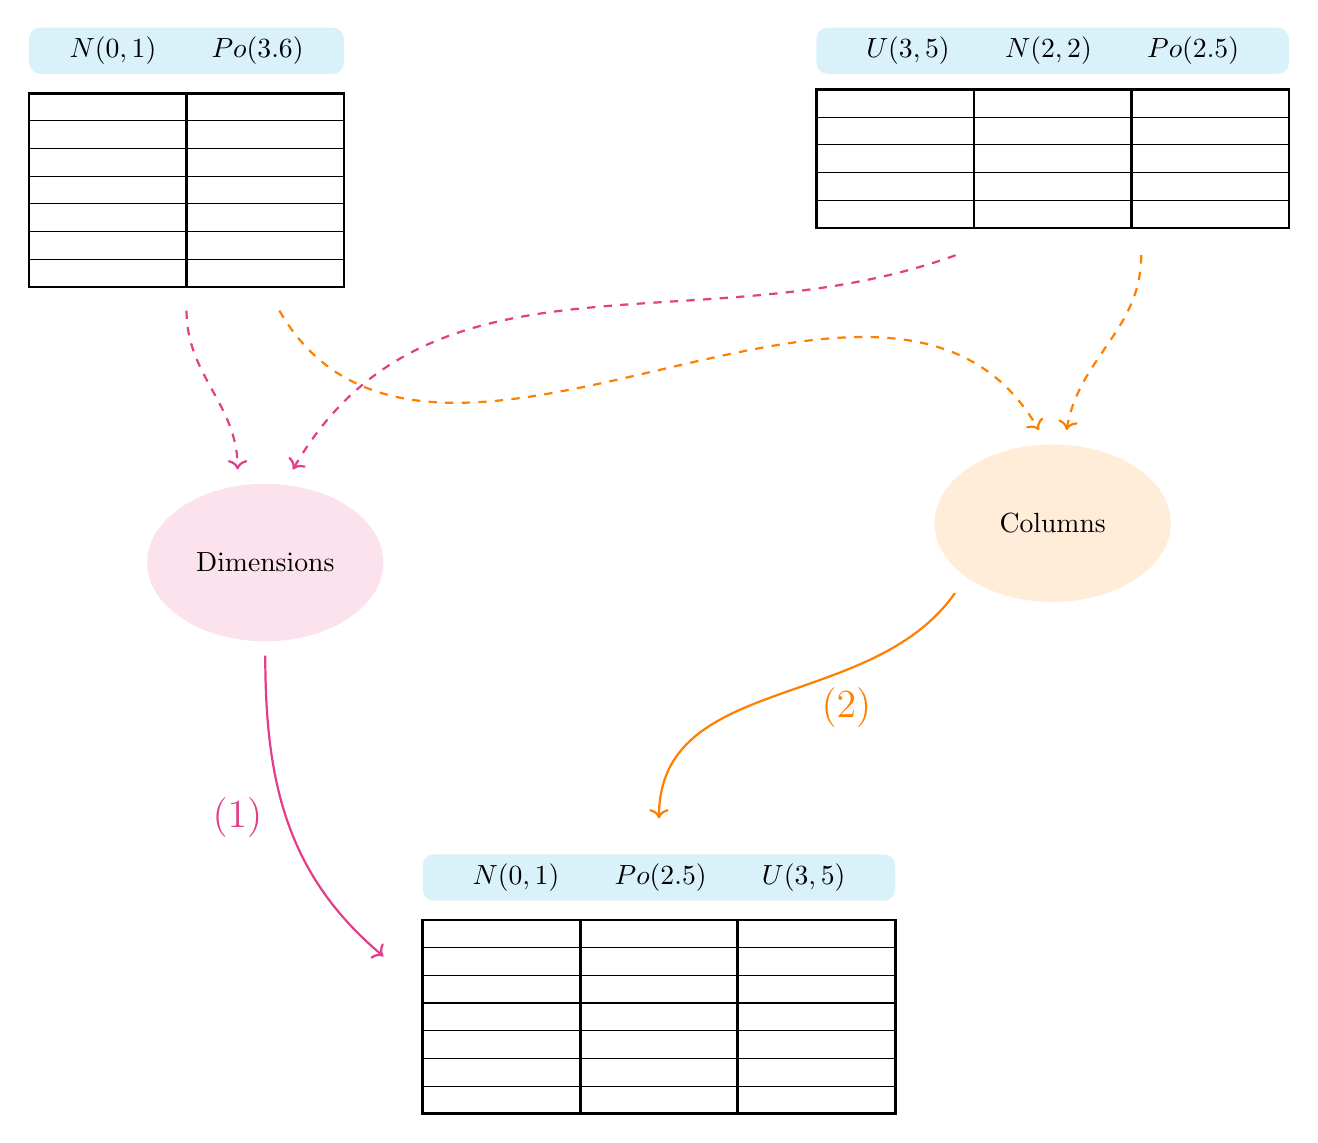
\begin{tikzpicture}

    % First individual
    \path (-2, 1.5) pic {fullcolumn=7}
          (0, 1.5) pic {fullcolumn=7};

    \node (parent1) at (-2, 1.5) {};
    \node[fill=cyan!15, minimum width=4cm, rounded corners] (info1) at (-2, 4.5)
        {\(N(0, 1) \qquad Po(3.6)\)};

    % Second individual
    \path (8, 2.25) pic {fullcolumn=5}
          (10, 2.25) pic {fullcolumn=5}
          (12, 2.25) pic {fullcolumn=5};

    \node (parent2) at (10, 1.5) {};
    \node[fill=cyan!15, minimum width=6cm, rounded corners] (info2) at (9, 4.5)
        {\(U(3, 5) \qquad N(2, 2) \qquad Po(2.5)\)};

    % Pools
    \node[%
        ellipse,
        fill=magenta!15,
        minimum width=3cm,
        minimum height=2cm
    ] (dims) at (-1, -2) {Dimensions};
    \node[%
        ellipse,
        fill=orange!15,
        minimum width=3cm,
        minimum height=2cm
    ] (cols) at (9, -1.5) {Columns};

    % Connecting parents to pools
    \draw[->, dashed, orange, thick]%
        ([xshift=30pt, yshift=-5pt] parent1.south east)
        to [out=300, in=120] ([xshift=-5pt, yshift=5pt] cols.north);

    \draw[->, dashed, orange, thick]
        ([yshift=20pt, yshift=-5pt] parent2.south east)
        to [out=270, in=80] ([xshift=5pt, yshift=5pt] cols.north);

    \draw[->, dashed, magenta, thick]
        ([xshift=-60pt, yshift=15pt] parent2.south west)
        to [out=200, in=60]
        ([xshift=10pt, yshift=5pt] dims.north);
    \draw[->, dashed, magenta, thick]
        ([yshift=-5pt] parent1.south)
        to [out=270, in=90] ([xshift=-10pt, yshift=5pt] dims.north);


    % The new individual
    \path (3, -9) pic {fullcolumn=7}
          (5, -9) pic {fullcolumn=7}
          (7, -9) pic {fullcolumn=7};

    \node[fill=cyan!15, minimum width=6cm, rounded corners] at (4, -6)
        {\(N(0, 1) \qquad Po(2.5) \qquad U(3, 5)\)};

    % Connecting up
    \draw[->, magenta, thick]
        ([yshift=-5pt] dims.south)
        to [out=270, in=140]
        (0.5, -7)
        node[above=50pt,left=40pt] {\Large (1)};

    \draw[->, orange, thick]
        ([xshift=-5pt, yshift=-5pt] cols.south west)
        to [out=235, in=90]
        (4, -5.25)
        node[above=40pt, right=55pt] {\Large (2)};

\end{tikzpicture}

    }\vfill
}

\frame{%
    \vfill\alert{Mutation}\vfill
    \centering
    \resizebox{!}{.75\paperheight}{%
        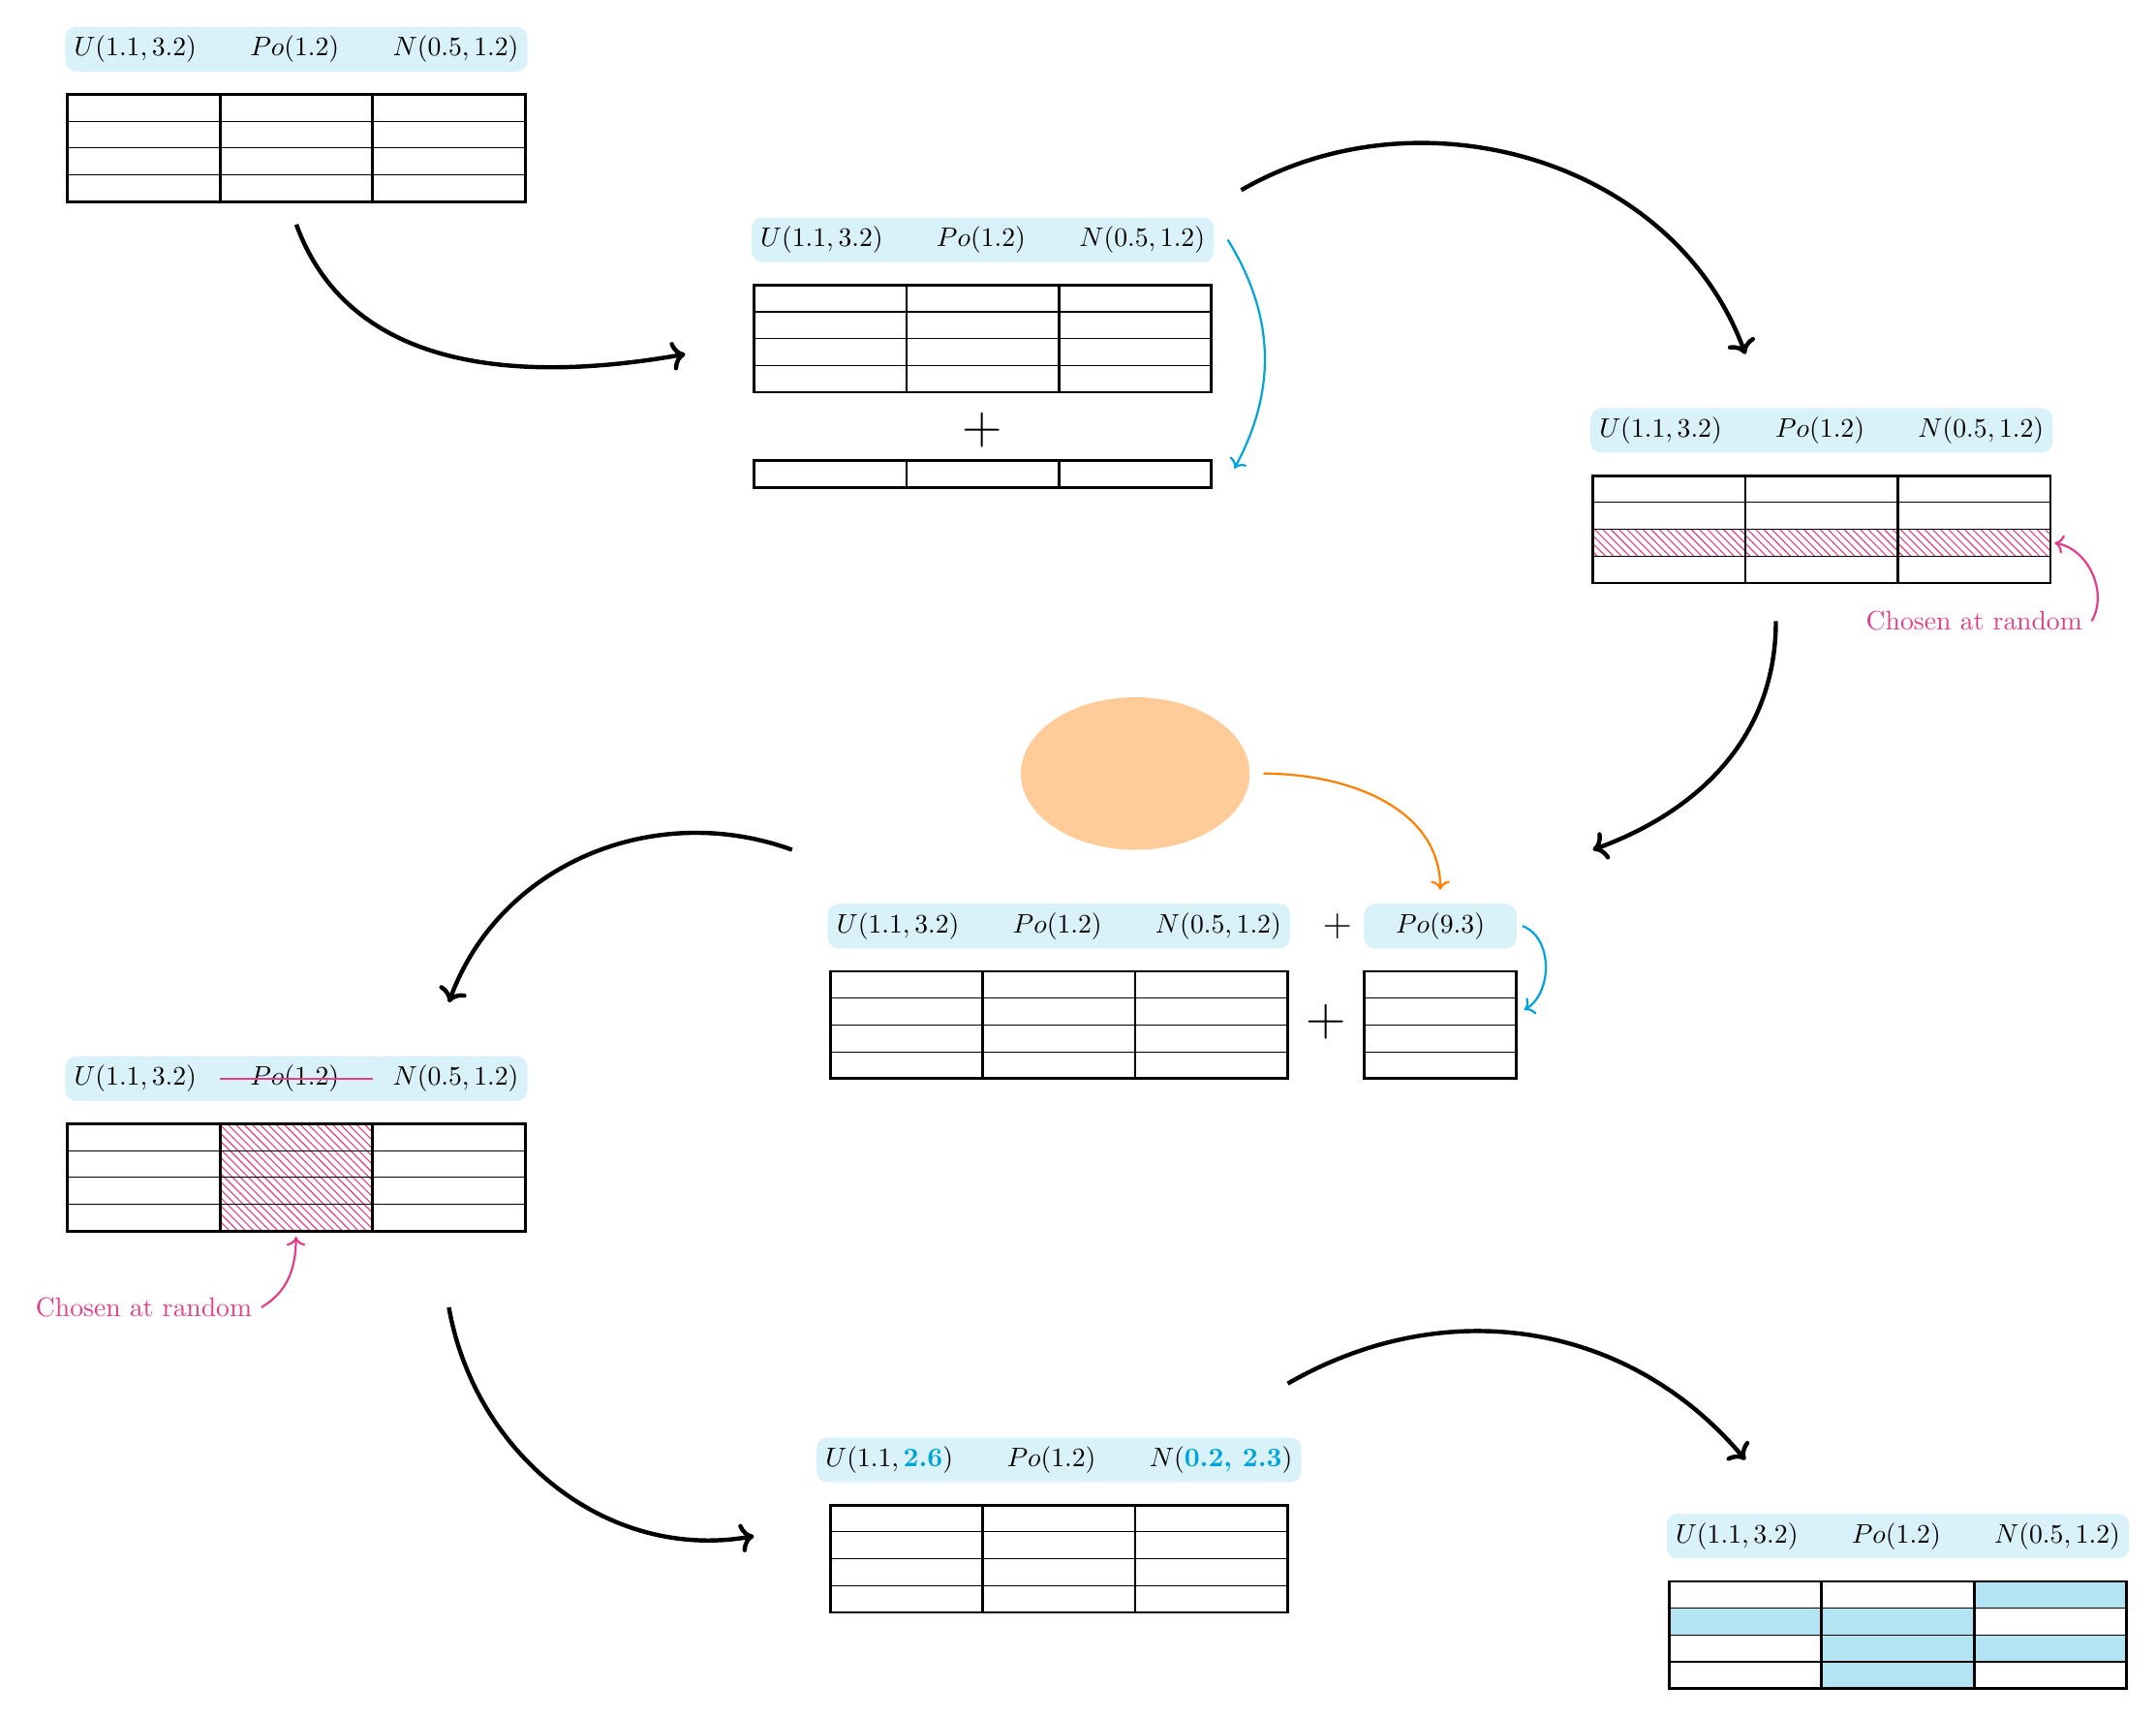
\begin{tikzpicture}

    % Individual
    \path (0, 1.5) pic {fullcolumn=4}
          (2, 1.5) pic {fullcolumn=4}
          (4, 1.5) pic {fullcolumn=4};

    \node (individual) at (1, 1.5) {};
    \node[fill=cyan!15, minimum width=6cm, rounded corners] at (1, 3.5)
        {\(U(1.1, 3.2) \qquad Po(1.2) \qquad N(0.5, 1.2)\)};

    % Adding a row
    \draw[->, black, ultra thick]
        ([yshift=-5pt] individual.south) to [out=290, in=190] (6.1, -0.5);

    \path (9, -1) pic {fullcolumn=4}
          (11, -1) pic {fullcolumn=4}
          (13, -1) pic {fullcolumn=4};
 
    \node[fill=cyan!15, minimum width=6cm, rounded corners] (r-info) at (10, 1)
        {\(U(1.1, 3.2) \qquad Po(1.2) \qquad N(0.5, 1.2)\)};

    \path (9, -2.25) pic {fullcolumn=1}
          (11, -2.25) pic {fullcolumn=1}
          (13, -2.25) pic {fullcolumn=1};

    \node (new-row) at (13, -2) {};
    \node (row-plus) at (10, -1.5) {\huge\(+\)};

    \draw[->, cyan, thick]
        ([xshift=5pt] r-info.east)
        to [bend left=30]
        ([xshift=5pt] new-row.east);


    % Deleting a row
    \draw[->, black, ultra thick]
        ([xshift=10pt, yshift=10pt] r-info.north east)
        to [out=30, in=110] (20, -0.5);

    \fill[pattern=north west lines, pattern color=magenta]
        (17.99, -3.15) rectangle (24, -2.8)
        node[right=80pt, midway] (row-remove) {};

    \path (20, -3.5) pic {fullcolumn=4}
          (22, -3.5) pic {fullcolumn=4}
          (24, -3.5) pic {fullcolumn=4};

    \node[fill=cyan!15, minimum width=6cm, rounded corners] at (21, -1.5)
    {\(U(1.1, 3.2) \qquad Po(1.2) \qquad N(0.5, 1.2)\)};

    \node (delete-row) at (23, -4) {\color{magenta} Chosen at random};

    \draw[->, magenta, thick]
        (delete-row.east) to [out=60, in=-10] (row-remove.east);


    % Adding a column
    \draw[->, black, ultra thick]
        (20.4, -4) to [out=270, in=20] (18, -7);

    \node[%
        ellipse,
        fill=orange!40,
        minimum width=3cm,
        minimum height=2cm
    ] (dists) at (12, -6) {};

    \path (10, -10) pic {fullcolumn=4}
          (12, -10) pic {fullcolumn=4}
          (14, -10) pic {fullcolumn=4};
 
    \node[fill=cyan!15, minimum width=6cm, rounded corners] at (11, -8)
        {\(U(1.1, 3.2) \qquad Po(1.2) \qquad N(0.5, 1.2)\)};

    \node (info-plus) at (14.65, -8) {\Large\(+\)};
    \node (col-plus) at (14.5, -9.25) {\huge\(+\)};

    \path (17, -10) pic {fullcolumn=4};
    \node[fill=cyan!15, minimum width=2cm, rounded corners] (c-info) at (16, -8)
        {\(Po(9.3)\)};

    \draw[->, orange, thick]
        ([xshift=5pt] dists.east)
        to [out=0, in=90]
        ([yshift=5pt] c-info.north);

    \draw[->, cyan, thick]
        ([xshift=2pt] c-info.east)
        to [out=-20, in=30]
        (17.1, -9.1);


    % Deleting a column
    \draw[->, black, ultra thick]
        (7.5, -7) to [out=160, in=70] (3, -9);

    \fill[pattern=north west lines, pattern color=magenta]
        (-0.01, -12) rectangle (2, -10.6)
        node[below=15pt, midway] (col-remove) {};

    \path (0, -12) pic {fullcolumn=4}
          (2, -12) pic {fullcolumn=4}
          (4, -12) pic {fullcolumn=4};
    \node[fill=cyan!15, minimum width=6cm, rounded corners] at (1, -10)
        {\(U(1.1, 3.2) \qquad Po(1.2) \qquad N(0.5, 1.2)\)};

    \draw[thick, magenta] (0, -10) -- (2, -10);

    \node (delete-col) at (-1, -13) {\color{magenta} Chosen at random};
    \draw[->, magenta, thick]
        (delete-col.east) to [out=30, in=270] (col-remove.south);


    % Mutate column parameters
    \draw[->, black, ultra thick]
        (3, -13) to [out=280, in=190] (7, -16);

    \path (10, -17) pic {fullcolumn=4}
          (12, -17) pic {fullcolumn=4}
          (14, -17) pic {fullcolumn=4};

    \node[fill=cyan!15, minimum width=6cm, rounded corners] at (11, -15)
        {\(%
            U(1.1, \textbf{\textcolor{cyan}{2.6}})
            \qquad Po(1.2) \qquad
            N(\textbf{\textcolor{cyan}{0.2, 2.3}})
        \)};


    % Mutate values
    \draw[->, black, ultra thick]
        (14, -14) to [out=30, in=130] (20, -15);


    \fill[cyan!30] (19, -17.3) rectangle (23, -16.95);

    \fill[cyan!30] (21, -18) rectangle (23, -17.3);
    
    \fill[cyan!30] (23, -16.95) rectangle (25, -16.6);
    \fill[cyan!30] (23, -17.65) rectangle (25, -17.3);

    \path (21, -18) pic {fullcolumn=4}
          (23, -18) pic {fullcolumn=4}
          (25, -18) pic {fullcolumn=4};

    \node[fill=cyan!15, minimum width=6cm, rounded corners] at (22, -16)
        {\(U(1.1, 3.2) \qquad Po(1.2) \qquad N(0.5, 1.2)\)};

\end{tikzpicture}

    }\vfill
}


\section{Some example use cases}

\frame{%
    \alert{Maximise}
    \[
        f: \mathbb{R}^n \times \mathbb{R}^n \to \mathbb{R},\qquad
        f(A, B) = Var(A) - \max_i \left|B_i - 1\right|
    \]
}

\frame{%
    \makebox[\linewidth]{%
        \includegraphics[width=.9\paperwidth]{../img/circle/fitness.pdf}
    }
}

\frame{%
    \makebox[\linewidth]{%
        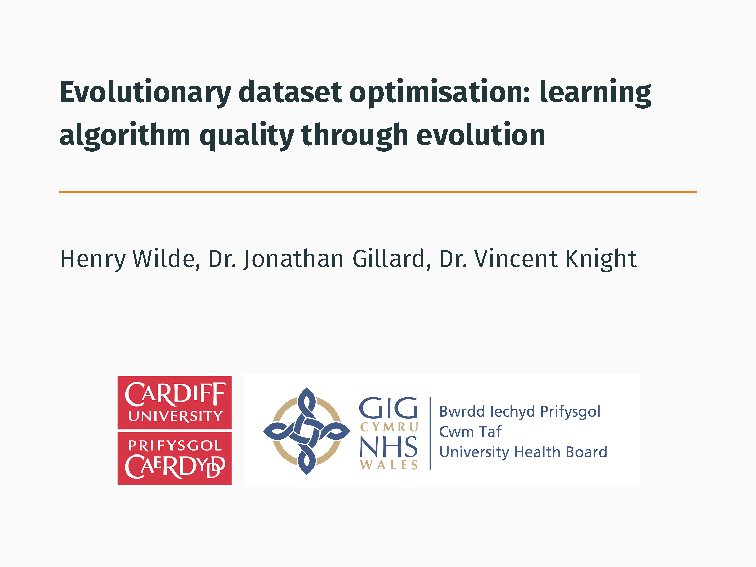
\includegraphics[width=.9\paperwidth]{../img/circle/main.pdf}
    }
}


\frame{%
    Given a set of \(k\) \alert{dissimilarity} measures:
    \[
        f_1, \ldots, f_k: \mathbb{R}^n \times \mathbb{R}^n \to \mathbb{R}
    \]

    \alert{Minimise} their sum
}

\frame{%
    \makebox[\linewidth]{%
        \includegraphics[width=.9\paperwidth]{../img/anscombe/fitness.pdf}
    }
}

\frame{%
    \centering{%
        \(X\) Mean: 5 \hfill%
        \(Y\) Mean: 7 \hfill%
        \(X\) Std.: 4.7 \hfill%
        \(Y\) Std.: 4.1 \hfill%
        Corr.: 0.8
    }\vfill

    \begin{minipage}{\linewidth}
        \hspace*{-30mm}
        \includegraphics[height=.4\paperheight]{../img/anscombe/best_0.pdf}%
        \hspace*{-30mm}\includegraphics[height=.4\paperheight]{../img/anscombe/best_1.pdf}
    \end{minipage}
    \begin{minipage}{\linewidth}
        \hspace*{-30mm}
        \includegraphics[height=.4\paperheight]{../img/anscombe/best_2.pdf}%
        \hspace*{-30mm}\includegraphics[height=.4\paperheight]{../img/anscombe/best_3.pdf}
    \end{minipage}
}



\hammerpage%




\frame{%
    \centering
    \Huge{\texttt{\$ pip install edo}}
}

\frame{%
    Henry Wilde
        \begin{itemize}
            \item[] \alert{Twitter:} @daffidwilde
            \item[] \alert{Email:} wildehd@cardiff.ac.uk
            \item[] \alert{Repository:} \url{%
                https://github.com/daffidwilde/edo
            }
            \item[] \alert{Documentation:} \url{https://edo.readthedocs.io}\\
        \end{itemize}

    Paper in preparation:
        \begin{itemize}
            \item[]\textit{%
                ``Evolutionary Dataset Optimisation: understanding algorithm
                quality through evolution''
            }
        \end{itemize}
}

\end{document}
